\documentclass[10pt]{article}
\usepackage{icmlko}

\icmlmeta{IP 파운데이션 월드모델}{267}{날짜가 아니었다}{코호트를 통제하면 달력은 41\% 무너지고 모형은 1\% 준다 --- 누적 라벨 걱정의 크기를 처음으로 쟀다}

\begin{document}

\twocolumn[
\icmlheader

\begin{abstract}
노트 266의 훑기가 축 0 개로 끝나면서 남은 깊은 갈래는 하나였다 --- 노트 209의
\textbf{누적 라벨}. 라벨이 연재 시작부터 쌓이면 ``언제 나왔나''가 곧 라벨이
되고, 그러면 판 0.484 의 상당 부분이 달력일 수 있다. 먼저 고칠 수 있는지
봤다: \textbf{못 고친다} --- 고정 창 라벨이 레코드에 있는 도메인은 게임뿐이고
(\texttt{y\_w30}), 그것은 노트 210이 이미 적용해 연도 상관이 $-$0.071 로
깨끗하다. 나머지 여덟은 새로 긁어야 한다. 그래서 \emph{고치는} 대신
\textbf{크기를 쟀다} --- 유보를 반년 코호트로 잘라 코호트 \emph{안에서만}
채점한다. 코호트 안에서는 모두가 같은 시기에 나왔으므로 날짜가 설명력을
잃는다. \textbf{결과가 분명하다}: 달력 기준선(``$-$시작일'' 하나)이 0.2287
$\to$ \textbf{0.1352}로 \textbf{41\% 무너지는데} 모형은 0.4725 $\to$
\textbf{0.4679}로 \textbf{1\%만} 준다. 노트 209가 옛 판에서 본 것이 지금 판
--- 축 스물셋, 새는 축 둘을 막은 뒤 --- 에서도 그대로다. \textbf{모형의
우위는 날짜에서 안 온다.} 도메인별로도 여덟 중 일곱이 같고, 하나만 다르다:
\textbf{도서는 달력(0.5615)이 모형(0.3480)을 이긴다.} 코호트 안에서는
뒤집히지만(0.3949 대 0.1814) 그대로 두면 ``$-$시작일'' 하나가 우리 모형보다
낫다. 노트 253 · 254가 도서를 두 번 짚었는데(제 학습이 해로운 유일한
도메인) 세 번째 얼굴이다. \textbf{누적 라벨은 여전히 숙제이지만 크기를
알았다} --- 기준선을 부풀릴 뿐 모형의 값을 만들지는 않는다.
\end{abstract}
]

\section{고칠 수 있나 --- 없다}

노트 209는 라벨이 누적인 도메인이 여섯이고 ``$-$시작일'' 하나로 판이 0.2513
이라고 적었다. 처방도 적어 뒀다 --- ``다음 수집 때 라벨을 고정 창으로''.

레코드를 열어 고정 창 후보를 찾았다.

\begin{center}\small
\begin{tabular}{ll}
\hline
도메인 & 라벨 관련 필드 \\
\hline
\textbf{게임} & \texttt{y\_raw} · \texttt{y\_positive} ·
  \textbf{\texttt{y\_w30}} · \texttt{y\_w30\_truncated} \\
웹툰 & \texttt{y\_favorite} \\
펀딩 & \texttt{y\_backers} \\
도서 & (\texttt{sales\_point}) \\
\hline
\end{tabular}
\end{center}

\textbf{게임만 있다.} 그리고 그것은 노트 210이 이미 적용했다 ---
\texttt{fixaxes.LABEL\_FIX} 가 게임 라벨을 \texttt{y\_w30} 으로 갈아 끼우고
있고, 지금 판의 게임 라벨은 \texttt{y\_w30} 과 상관 $+$1.000 · 시작연도와
$-$0.071 이다. 나머지 여덟은 새로 긁어야 하고, 그건 이 노트에서 못 한다.

\section{그러면 크기를 재자}

고칠 수 없으면 \emph{얼마나 나쁜지}라도 알아야 한다. 노트 209가 쓴 방법이
있다 --- 유보를 반년 코호트로 자르고 \textbf{코호트 안에서만} 채점한다.
코호트 안에서는 모두가 같은 시기에 나왔으므로 ``언제 나왔나''가 힘을 잃는다.

\begin{figure}[t]
\centering
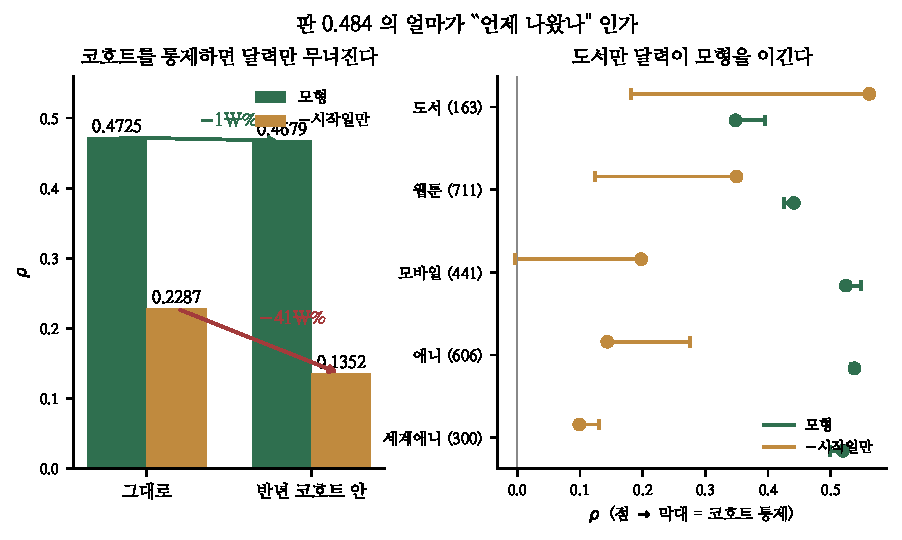
\includegraphics[width=\columnwidth]{figs/cohort.pdf}
\caption{왼쪽 --- 판 수준. 오른쪽 --- 도메인별. 점에서 막대로 가는 것이
코호트 통제다.}
\end{figure}

\begin{center}\small
\begin{tabular}{lrr}
\hline
 & 그대로 & 반년 코호트 안 \\
\hline
\textbf{모형} & 0.4725 & \textbf{0.4679} ($-$1\%) \\
\textbf{$-$시작일만} & 0.2287 & \textbf{0.1352} ($-$41\%) \\
\hline
\end{tabular}
\end{center}

\textbf{달력은 41\% 무너지고 모형은 1\% 준다.} 노트 209가 옛 판(축 다섯,
판 0.44 언저리)에서 본 것과 같은 그림이 지금 판 --- 축 스물셋, 노트 262 ·
263이 새는 축 둘을 막은 뒤 --- 에서도 나온다.

읽는 법을 분명히 해 두자. 이것은 ``판 0.484 중 0.23 이 달력''이라는 뜻이
\emph{아니다}. 달력과 모형은 겹치는 부분이 있고, 코호트 통제는 그 겹침을
걷어낸다. 걷어낸 뒤 \textbf{달력은 거의 남지 않고 모형은 거의 다 남는다}는
것이 결과다.

\section{도서 하나가 다르다}

\begin{center}\small
\begin{tabular}{lrrrr}
\hline
 & \multicolumn{2}{c}{그대로} & \multicolumn{2}{c}{코호트 안} \\
도메인 & 모형 & 달력 & 모형 & 달력 \\
\hline
\textbf{도서} & 0.3480 & \textbf{0.5615} & 0.3949 & 0.1814 \\
웹툰 & 0.4413 & 0.3497 & 0.4256 & 0.1247 \\
애니 & 0.5377 & 0.1436 & 0.5316 & 0.2750 \\
모바일 & 0.5241 & 0.1976 & 0.5477 & $-$0.0035 \\
세계애니 & 0.5194 & 0.0990 & 0.4992 & 0.1305 \\
팝업 & 0.3205 & $-$0.1129 & 0.2889 & --- \\
펀딩 & 0.2292 & $-$0.0120 & 0.2315 & --- \\
\hline
\end{tabular}
\end{center}

일곱은 모형이 달력을 크게 이기고 코호트 통제에도 안 흔들린다. \textbf{도서만
반대다} --- ``$-$시작일'' 하나가 0.5615 로 우리 모형(0.3480)을 \emph{이긴다}.
코호트 안에서는 뒤집히지만(0.3949 대 0.1814), 그대로 두면 \textbf{날짜 한
줄이 축 스물셋보다 낫다.}

이 실험실이 도서를 세 번째로 짚는다. 노트 252가 여지 $+$0.177 로 1위라
했고, 노트 253이 ``제 학습 자료가 제 도메인을 해치는 유일한 도메인''임을
쟀고(덜어 내면 좋아진다), 노트 254가 아홉 중 도서만 그렇다고 확인했다.
이번은 그 셋과 같은 뿌리로 보인다 --- 도서 레코드는 베스트셀러 목록
스크랩이라 ``2020년 이전''이 ``지금도 잘 팔리는 옛 책''이고, 그러면 날짜가
곧 라벨이다.

\section{숙제의 크기를 알았다}

노트 209의 처방(고정 창 라벨)은 여전히 옳고 여전히 못 했다. 바뀐 것은
\textbf{우선순위}다.

\begin{itemize}
\item 고정 창으로 바꾸면 \textbf{기준선이 크게 내려간다}(달력 0.229 $\to$
0.135 쪽으로) --- 즉 판 $\rho$ 의 절대값이 지금보다 낮아 보일 것이다.
\item 그런데 \textbf{모형은 거의 안 움직인다}(1\%). 우리가 재고 있는 것은
이미 대부분 날짜가 아니다.
\item 그러니 고정 창 수집은 \emph{점수를 정직하게 만드는} 일이지
\emph{모형을 좋게 만드는} 일이 아니다. 노트 213의 공휴일, 노트 262 · 263의
새는 축과 같은 종류다.
\end{itemize}

\paragraph{남은 것}
\begin{center}\small
\begin{tabular}{ll}
\hline
갈래 & 왜 \\
\hline
도서 & 네 번째 얼굴. 달력이 모형을 이긴다 \\
고정 창 수집 & 여덟 도메인. 점수를 정직하게 하는 일 \\
\texttt{SOURCE} 채우기 & 20/45 쌍 \\
코호트를 판정에 & 지금은 진단이다. 순위 기준으로 쓰면? \\
\hline
\end{tabular}
\end{center}

\paragraph{규약} ``라벨이 오염됐을 것''이라고 걱정할 때 \textbf{코호트 안에서
다시 재 본다.} 걱정의 크기가 숫자로 나온다 --- 이번엔 모형 쪽 1\%,
기준선 쪽 41\% 였다. 노트 253의 ``덜어 내 본다'' · 노트 259의 ``잡음을
먹여 본다'' · 노트 261의 ``떼어 본다''에 이어 네 번째 한 줄짜리 검정이다.

\end{document}
